% ============================================================
% Lesson 4-1: Inverse Variation / Reciprocal Function
% Algebra 2 — Savvas enVision — Student Lesson Packet
% Compile with: pdflatex envAlg2_04_01_LessonPacket.tex
% ============================================================
\documentclass[11pt]{article}

% -------- Packages --------
\usepackage[letterpaper,margin=0.75in]{geometry}
\usepackage{amsmath,amssymb,amsfonts}
\usepackage{array}
\usepackage{tabularx}
\usepackage{booktabs}
\usepackage{enumitem}
\usepackage{xcolor}
\usepackage[most]{tcolorbox}
\usepackage{tikz}
\usepackage{pgfplots}
\pgfplotsset{compat=1.18}
\usepackage{graphicx}
\usepackage{parskip}
\usepackage{fancyhdr}

% -------- Colors (Savvas-ish palette) --------
\definecolor{savvasblue}{HTML}{2E75B6}
\definecolor{savvaslight}{HTML}{DEEBF7}
\definecolor{highlightyellow}{HTML}{FFF176}
\definecolor{framegray}{HTML}{BFBFBF}

% -------- Section headers as "highlighted" bars --------
\newcommand{\sectionbar}[1]{%
  \vspace{0.4em}%
  \noindent\colorbox{highlightyellow}{\parbox{\dimexpr\linewidth-2\fboxsep}{\textbf{#1}}}%
  \vspace{0.2em}%
}

% -------- Example / Try It heading --------
\newcommand{\examplehead}[1]{%
  \vspace{0.5em}%
  \noindent\textbf{\large #1}%
  \vspace{0.3em}%
}

% -------- Quick Guide / Concept box --------
\newtcolorbox{quickbox}[1]{
  enhanced, colback=savvaslight, colframe=savvasblue,
  boxrule=0.6pt, arc=2pt,
  left=8pt, right=8pt, top=6pt, bottom=6pt,
  title={\textbf{#1}}, coltitle=white, colbacktitle=savvasblue,
  fonttitle=\bfseries
}

% -------- Sentence-frame table (2x2) --------
\newcommand{\frametable}[4]{%
  \begin{center}
  \renewcommand{\arraystretch}{1.4}
  \begin{tabularx}{0.85\linewidth}{|>{\itshape}X|>{\itshape}X|}
    \hline
    \textit{``#1''} & \textit{``#2''} \\ \hline
    \textit{``#3''} & \textit{``#4''} \\ \hline
  \end{tabularx}
  \end{center}
}

% -------- Blank student graph grid --------
% Usage: \blankgrid{scale}{xmin}{xmax}{ymin}{ymax}
\newcommand{\blankgrid}[5]{%
\begin{center}
\begin{tikzpicture}[scale=#1]
  \draw[step=0.5,framegray,very thin] (#2,#4) grid (#3,#5);
  \draw[step=1,gray!60,thin]          (#2,#4) grid (#3,#5);
  \draw[->,thick] (#2,0) -- (#3,0) node[right] {\small $x$};
  \draw[->,thick] (0,#4) -- (0,#5) node[above] {\small $y$};
  \foreach \x in {#2,...,#3}{%
    \draw (\x,-0.1) -- (\x,0.1);
  }
  \foreach \y in {#4,...,#5}{%
    \draw (-0.1,\y) -- (0.1,\y);
  }
\end{tikzpicture}
\end{center}
}

% -------- Page style --------
\pagestyle{fancy}
\fancyhf{}
\fancyfoot[R]{\footnotesize Lesson 4-1 \textbullet{} Inverse Variation / Reciprocal Function \textbullet{} p.~\thepage}
\renewcommand{\headrulewidth}{0pt}

\setlength{\parindent}{0pt}

% ============================================================
\begin{document}
% ============================================================

% -------- Student header --------
\noindent
\begin{tabular}{@{}p{0.45\linewidth}p{0.25\linewidth}p{0.25\linewidth}@{}}
Name\underline{\hspace{\linewidth}} &
Date\underline{\hspace{\linewidth}} &
Section\underline{\hspace{\linewidth}} \\
\end{tabular}

\vspace{0.6em}
\begin{center}
  {\Large\bfseries Lesson 4-1: Inverse Variation / Reciprocal Function}
\end{center}

% -------- Objectives table --------
\renewcommand{\arraystretch}{1.4}
\begin{tabularx}{\linewidth}{|>{\bfseries\raggedright\arraybackslash}p{1.5in}|X|}
  \hline
  Math Objective &
  Identify and use Inverse Variation. Graph reciprocal functions. \\ \hline
  Language Objective &
  Students will be able to describe why a relation is an inverse variation with the support of sentence frames. \\ \hline
  Essential Understanding &
  The reciprocal function is used to model inverse variation, which is a proportional relationship between 2 variables such that when one increases, the other decreases. \\ \hline
\end{tabularx}

% ============================================================
\sectionbar{MODEL AND REASON}
% ============================================================

A pump is emptying a water tank. Here are some different pumping rates and the times it takes to empty the tank:

\begin{center}
\renewcommand{\arraystretch}{1.3}
\begin{tabular}{|>{\centering\arraybackslash}p{1.5in}|>{\centering\arraybackslash}p{1.2in}|}
  \hline
  \textbf{Pump Rate (gal/min)} & \textbf{Time (min)} \\ \hline
  120 & 40  \\ \hline
  80  & 60  \\ \hline
  60  & 80  \\ \hline
  40  & 120 \\ \hline
      &     \\ \hline
      &     \\ \hline
\end{tabular}
\end{center}

\begin{itemize}[leftmargin=*]
  \item What happens to the time when the pump rate increases?
\end{itemize}
\frametable%
{When the pump rate goes \textbf{up}, the time goes \underline{\hspace{0.8in}}.}%
{A bigger rate means the time is \underline{\hspace{0.8in}}.}%
{I notice the time gets \underline{\hspace{0.8in}} when the rate is higher.}%
{As the rate increases, the time seems to \underline{\hspace{0.8in}}.}

\begin{itemize}[leftmargin=*]
  \item Try multiplying \textbf{rate} $\times$ \textbf{time} for two rows. What do you notice?
\end{itemize}
\vspace{0.6in}
\frametable%
{For the second row, the product is \underline{\hspace{0.6in}}.}%
{The products are \underline{\hspace{0.5in}} and \underline{\hspace{0.5in}}, so they are \underline{\hspace{0.6in}}.}%
{I notice the product stays \underline{\hspace{0.8in}}.}%
{The product does/does not change because \underline{\hspace{1.0in}}.}

\begin{itemize}[leftmargin=*]
  \item What would happen with a pump rate of 200 gal/min? Explain your thinking.
\end{itemize}
\vspace{0.6in}
\frametable%
{If the rate is 200 gal/min, I think the time would be \underline{\hspace{0.5in}} because \underline{\hspace{0.8in}}.}%
{A faster pump means the time should be \underline{\hspace{0.8in}}.}%
{At 200 gal/min, the time might be around \underline{\hspace{0.5in}} minutes.}%
{I predict the time will be \underline{\hspace{0.5in}} since the pattern shows \underline{\hspace{0.8in}}.}

\begin{itemize}[leftmargin=*]
  \item Pick \textbf{2} new pump rates and estimate how long it would take to empty the tank.
\end{itemize}
\vspace{0.8in}

% ============================================================
\begin{quickbox}{QUICK GUIDE --- Inverse Variation}
\textbf{Definition.}\ Two variables show \textbf{inverse variation} if their product is constant:
\[
  xy = k
\]
This can also be written as:
\[
  y = \frac{k}{x}
\]

\textbf{Key Features}
\begin{itemize}[leftmargin=*,itemsep=2pt]
  \item As one variable \textbf{increases}, the other \textbf{decreases}.
  \item The product $xy$ stays \textbf{constant}.
  \item The graph looks like a \textbf{reciprocal curve} $\rightarrow$
\end{itemize}

\begin{center}
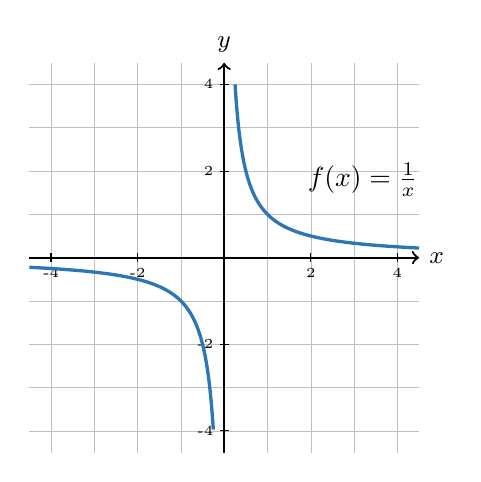
\begin{tikzpicture}[scale=0.55]
  \draw[step=1,framegray,very thin] (-4.5,-4.5) grid (4.5,4.5);
  \draw[->,thick] (-4.5,0) -- (4.5,0) node[right] {\small $x$};
  \draw[->,thick] (0,-4.5) -- (0,4.5) node[above] {\small $y$};
  \foreach \x in {-4,-2,2,4}
    \draw (\x,-0.1) -- (\x,0.1) node[below=2pt] {\tiny \x};
  \foreach \y in {-4,-2,2,4}
    \draw (-0.1,\y) -- (0.1,\y) node[left=2pt] {\tiny \y};
  \draw[savvasblue,very thick,samples=200,domain=0.25:4.5] plot (\x,{1/\x});
  \draw[savvasblue,very thick,samples=200,domain=-4.5:-0.25] plot (\x,{1/\x});
  \node at (3.2,1.8) {$f(x)=\tfrac{1}{x}$};
\end{tikzpicture}
\end{center}
\end{quickbox}

% ============================================================
\examplehead{\colorbox{highlightyellow}{EXAMPLE 1 --- Identify Inverse Variation}}

Does the table represent an inverse variation?

\begin{center}
\renewcommand{\arraystretch}{1.4}
\begin{tabular}{|c|c|c|c|c|c|}
  \hline
  $x$  & 1  & 2 & 3 & 4 & 6 \\ \hline
  $y$  & 12 & 6 & 4 & 3 & 2 \\ \hline
  $xy$ & \rule{0.5in}{0.4pt} & \rule{0.5in}{0.4pt} & \rule{0.5in}{0.4pt} & \rule{0.5in}{0.4pt} & \rule{0.5in}{0.4pt} \\ \hline
\end{tabular}
\end{center}

Compute the \textit{products}\ldots

\textbf{Yes.} The product is constant $\rightarrow$ inverse variation.

% ============================================================
\examplehead{TRY IT 1}

Determine whether each table represents an inverse variation.

\begin{center}
\renewcommand{\arraystretch}{1.4}
\begin{tabular}{|c|c|c|c|c|c|c|}
  \hline
  $x$  & 1    & 2     & 3    & 5    & 6    & 15   \\ \hline
  $y$  & 25.5 & 12.75 & 8.50 & 5.10 & 4.25 & 1.70 \\ \hline
  $xy$ & & & & & & \\[0.9em] \hline
\end{tabular}
\end{center}

\vspace{0.3em}

\begin{center}
\renewcommand{\arraystretch}{1.4}
\begin{tabular}{|c|c|c|c|c|c|c|}
  \hline
  $x$  & 6.6 & 5.5 & 4.4 & 3.3 & 2.2 & 1.1 \\ \hline
  $y$  & 3   & 5   & 7   & 9   & 11  & 13  \\ \hline
  $xy$ & & & & & & \\[0.9em] \hline
\end{tabular}
\end{center}

% ============================================================
\examplehead{\colorbox{highlightyellow}{EXAMPLE 2 --- Write an Inverse Variation Equation}}

In an inverse variation, $x=10$ when $y=3$. Write the equation and find $y$ when $x=-6$.

\textbf{Step 1:} Find the constant $k$.
\[
  k = xy = (10)(3) = 30
\]

\textbf{Step 2:} Write the equation.
\[
  y = \frac{30}{x}
\]

\textbf{Step 3:} Substitute $x=-6$.
\[
  y = \frac{30}{-6} = -5
\]

% ============================================================
\examplehead{TRY IT 2}

If $x=6$ when $y=16$:

\begin{center}
\begin{tabular}{@{}p{2.0in}p{2.0in}p{2.0in}@{}}
  a.\ Find $k$. & b.\ Write the equation. & c.\ Find $y$ when $x=15$. \\[1.6in]
\end{tabular}
\end{center}

% ============================================================
\examplehead{\colorbox{highlightyellow}{EXAMPLE 3 --- Use an Inverse Variation Model}}

The number of downloaded games $n$ that can be stored on a video game system varies inversely with the average game size $s$ in gigabytes (GB).

A certain system can store \textbf{160 games} when the average game size is \textbf{2.0 GB}.

\textbf{A. Write an inverse equation that relates $n$ and $s$.}
\[
  n = \frac{k}{s}
  \qquad\Longrightarrow\qquad
  160 = \frac{k}{2.0}
  \qquad\Longrightarrow\qquad
  k = 320
\]
\[
  \boxed{\,n = \dfrac{320}{s}\,}
\]

\textbf{B. Use the inverse relationship to complete the table.}

\begin{center}
\renewcommand{\arraystretch}{1.4}
\begin{tabular}{|l|c|c|c|c|}
  \hline
  \textbf{Game Size (GB), $s$}   & 1.0 & 2.5 & 3.0 & 4.0 \\ \hline
  \textbf{Number of Games, $n$}  &     &     &     &     \\[0.6em] \hline
  $ns$                            & 320 & 320 & 320 & 320 \\ \hline
\end{tabular}
\end{center}

\textbf{C. Sketch a graph of this inverse relationship where $n > 0$.}

\blankgrid{0.35}{0}{10}{0}{10}

% ============================================================
\examplehead{TRY IT 3 --- Ice Cube Melting}

The time $t$ it takes for an ice cube to melt varies inversely with the air temperature $T$ in $^\circ$C. At \textbf{20\,$^\circ$C}, the ice melts in \textbf{20 minutes}. Write an inverse equation and find out how long it will take to melt at \textbf{30\,$^\circ$C}. Sketch a graph of this relationship.

\blankgrid{0.35}{0}{10}{0}{10}

% ============================================================
\begin{quickbox}{THE RECIPROCAL FUNCTION --- Key Features}
The reciprocal function is:
\[
  f(x) = \frac{1}{x}
\]

\textbf{Important Characteristics}
\begin{itemize}[leftmargin=*,itemsep=2pt]
  \item \textbf{Vertical asymptote:} $x = 0$
  \item \textbf{Horizontal asymptote:} $y = 0$
  \item \textbf{Domain:} all real numbers except $0$
  \item \textbf{Range:} all real numbers except $0$
  \item As $x \to 0^+,\ f(x) \to +\infty$
  \item As $x \to 0^-,\ f(x) \to -\infty$
  \item As $x \to \pm\infty,\ f(x) \to 0$
\end{itemize}
\end{quickbox}

% ============================================================
\examplehead{\colorbox{highlightyellow}{EXAMPLE 4 --- Transformations of the Reciprocal Function}}

Graph:
\[
  g(x) = \frac{1}{x-3} + 2
\]

\textbf{Transformations}
\begin{itemize}[leftmargin=*,itemsep=2pt]
  \item Shift \textbf{right 3} \quad + \quad Shift \textbf{up 2}
\end{itemize}

\textbf{Asymptotes}
\begin{itemize}[leftmargin=*,itemsep=2pt]
  \item Vertical: $x = 3$ \quad + \quad Horizontal: $y = 2$
\end{itemize}

\textbf{Domain \& Range}
\begin{itemize}[leftmargin=*,itemsep=2pt]
  \item Domain: $x \neq 3$ \qquad Range: $y \neq 2$
\end{itemize}

% -------- Reference graph of g(x) = 1/(x-3) + 2 --------
\begin{center}
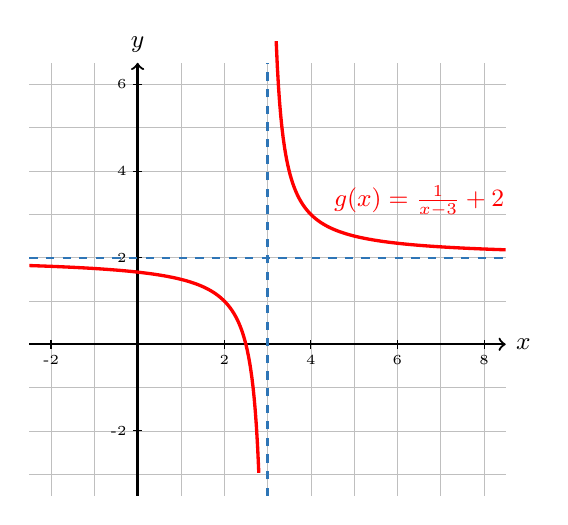
\begin{tikzpicture}[scale=0.55]
  \draw[step=1,framegray,very thin] (-2.5,-3.5) grid (8.5,6.5);
  \draw[->,thick] (-2.5,0) -- (8.5,0) node[right] {\small $x$};
  \draw[->,thick] (0,-3.5) -- (0,6.5) node[above] {\small $y$};
  \foreach \x in {-2,2,4,6,8}
    \draw (\x,-0.1) -- (\x,0.1) node[below=2pt] {\tiny \x};
  \foreach \y in {-2,2,4,6}
    \draw (-0.1,\y) -- (0.1,\y) node[left=2pt] {\tiny \y};
  % asymptotes
  \draw[dashed,savvasblue,thick] (3,-3.5) -- (3,6.5);
  \draw[dashed,savvasblue,thick] (-2.5,2) -- (8.5,2);
  % g(x) = 1/(x-3) + 2
  \draw[red,very thick,samples=200,domain=3.2:8.5] plot (\x,{1/(\x-3)+2});
  \draw[red,very thick,samples=200,domain=-2.5:2.8] plot (\x,{1/(\x-3)+2});
  \node[red] at (6.5,3.3) {\small $g(x)=\tfrac{1}{x-3}+2$};
\end{tikzpicture}
\end{center}

% ============================================================
\examplehead{TRY IT 4}

Graph:
\[
  g(x) = \frac{1}{x+2} - 4
\]

Identify:
\begin{itemize}[leftmargin=*,itemsep=2pt]
  \item Vertical asymptote
  \item Horizontal asymptote
  \item Domain
  \item Range
\end{itemize}

\blankgrid{0.35}{-6}{6}{-8}{4}

% ============================================================
\vspace{0.5em}
\begin{quickbox}{CONCEPT SUMMARY --- Inverse Variation and the Reciprocal Function}
\renewcommand{\arraystretch}{1.5}
\begin{tabularx}{\linewidth}{|>{\bfseries}p{0.9in}|X|X|}
  \hline
   & \textbf{Inverse Variation} & \textbf{Transformations of the Reciprocal Function} \\ \hline
  WORDS    &
    An inverse variation is a relation between two variables such that as one variable increases, the other decreases proportionally. &
    The reciprocal function models the inverse variation, $y = \frac{1}{x}$. Like other functions, it can be transformed. \\ \hline
  ALGEBRA  &
    $y = \dfrac{k}{x}$,\ where $k \neq 0$ &
    $y = \dfrac{a}{x-h} + k$ \\ \hline
  EXAMPLES &
    $y = \dfrac{1}{x}$; \ asymptotes: $x=0,\ y=0$ &
    $y = \dfrac{1}{x-4} - 2$; \ $h=4$, $k=-2$; \ parent shifted right 4, down 2; \ asymptotes: $x=4,\ y=-2$ \\ \hline
\end{tabularx}
\end{quickbox}

% ============================================================
\newpage
\begin{center}
  {\Large\bfseries Select Exercises}
\end{center}

\renewcommand{\arraystretch}{1.3}
\begin{tabularx}{\linewidth}{|X|X|}
\hline
\textbf{9.} \textcolor{red}{\textit{Generalize}} Just from looking at the table of values, how can you determine that the data do \textit{not} represent an inverse variation?
\vspace{0.3em}

\begin{center}
\begin{tabular}{|c|c|c|c|c|c|c|}
  \hline
  $x$ & $-2$ & 2 & 4 & 6  & 8  & 10 \\ \hline
  $y$ & $-6$ & 6 & 12& 18 & 24 & 30 \\ \hline
\end{tabular}
\end{center}
\vspace{0.2em}
\hfill \textit{\small DOK 1}
&
\vspace{1.8in}
\\ \hline
\textbf{16.} If $x$ and $y$ vary inversely and $x=3$ when $y=\tfrac{2}{3}$, what is the value of $y$ when $x=-1$? \\ \textsc{\small see example 2}
\vspace{0.2em}
\hfill \textit{\small DOK 1}
&
\vspace{1.8in}
\\ \hline
\textbf{17.} The wavelength, $w$, of a radio wave varies inversely with its frequency, $f$, as shown in the graph.
\vspace{0.3em}

\begin{center}
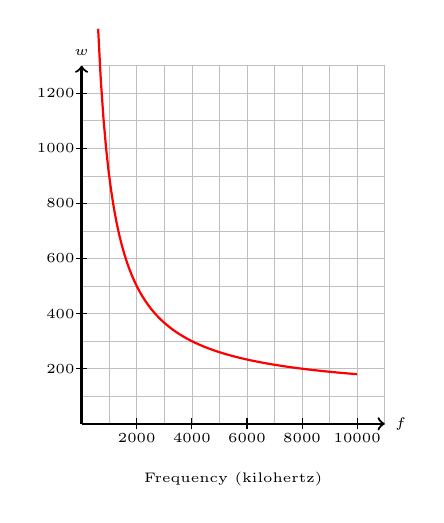
\begin{tikzpicture}[scale=0.35]
  \draw[step=1,framegray,very thin] (0,0) grid (11,13);
  \draw[->,thick] (0,0) -- (11,0) node[right] {\tiny $f$};
  \draw[->,thick] (0,0) -- (0,13) node[above] {\tiny $w$};
  \foreach \x/\lab in {2/2000,4/4000,6/6000,8/8000,10/10000}
    \draw (\x,-0.2) -- (\x,0.2) node[below=2pt] {\tiny \lab};
  \foreach \y/\lab in {2/200,4/400,6/600,8/800,10/1000,12/1200}
    \draw (-0.2,\y) -- (0.2,\y) node[left=1pt] {\tiny \lab};
  \draw[red,thick,samples=100,domain=0.6:10] plot (\x,{8/\x+1});
  \node at (5.5,-2) {\tiny Frequency (kilohertz)};
\end{tikzpicture}
\end{center}

A radio wave with a frequency of 1{,}000 kilohertz has a length of 300~m. What is the frequency when the wavelength is 375~m? \textsc{\small see example 3}
\vspace{0.2em}
\hfill \textit{\small DOK 2}
&
\vspace{2.2in}
\\ \hline
\textbf{19.} Graph $g(x) = \dfrac{1}{x-2} + 6$. What are the equations of the asymptotes? What are the domain and range? What are the intercepts? \textsc{\small see example 5}
\vspace{0.2em}
\hfill \textit{\small DOK 2}
&
\vspace{0.2em}
\begin{center}
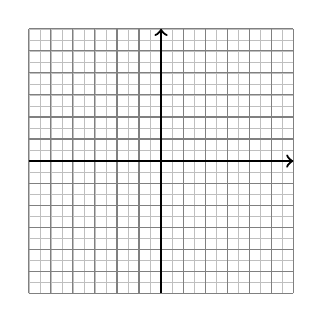
\begin{tikzpicture}[scale=0.28]
  \draw[step=0.5,framegray,very thin] (-6,-6) grid (6,6);
  \draw[step=1,gray,thin] (-6,-6) grid (6,6);
  \draw[->,thick] (-6,0) -- (6,0);
  \draw[->,thick] (0,-6) -- (0,6);
\end{tikzpicture}
\end{center}
\\ \hline
\textbf{25.} \textcolor{red}{\textbf{SAT/ACT}} In a given set of experiments, $t$ and $w$ always vary inversely. When $t=0.4$ seconds, $w=172.8$ grams. How much time has passed when $w=14.4$ grams?

\begin{tabular}{ll}
  \textcircled{A}~2.4\,s  & \textcircled{C}~27.648\,s  \\
  \textcircled{B}~4.8\,s  & \textcircled{D}~995.328\,s \\
\end{tabular}
\vspace{0.2em}
\hfill \textit{\small DOK 3}
&
\vspace{1.8in}
\\ \hline
\end{tabularx}

\end{document}
